% convex-polygon-vertex-diameter.tex

\documentclass[tikz]{standalone}
\usetikzlibrary{calc}

\begin{document}
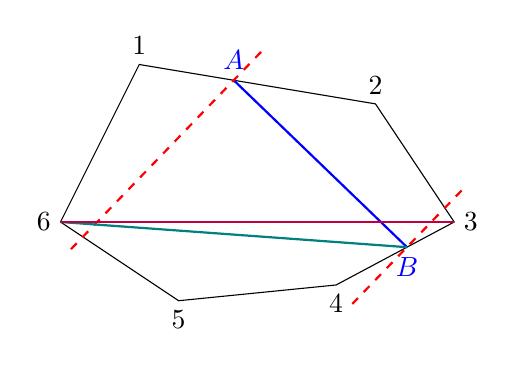
\begin{tikzpicture}
  \coordinate (1) at (1,2); 
  \coordinate (2) at (4, 1.5); 
  \coordinate (3) at (5,0); 
  \coordinate (4) at (3.5, -0.8); 
  \coordinate (5) at (1.5, -1);
  \coordinate (6) at (0,0);

  \path[draw] (6) node[left] {6}
    -- (5) node[below] {5}
    -- (4) node[below] {4}
    -- (3) node[right] {3}
    -- (2) node[above] {2}
    -- (1) node[above] {1}
    -- cycle;

  % A -- B
  \coordinate (A) at ($(1)!0.4!(2)$);
  \coordinate (B) at ($(3)!0.4!(4)$);
  \draw[thick, blue] (A) node[above] {$A$} -- (B) node[below] {$B$};

  % \pause
  % B -- 6
  \draw[thick, dashed, red, shorten >= -2cm, shorten <= -0.5cm] (A) -- ($(A)!1cm!-90:(B)$);
  \draw[thick, teal] (B) -- (6);

  % \pause
  % 6 -- 3
  \draw[thick, dashed, red, shorten >= 2cm, shorten <= -1.0cm] (B) -- ($(B)!1cm!-90:(A)$);
  \draw[thick, purple] (6) -- (3);
\end{tikzpicture}
\end{document}